\documentclass[12pt,t]{beamer}
\usepackage{graphicx}
\setbeameroption{hide notes}
\setbeamertemplate{note page}[plain]
\usepackage{xmpmulti}
\usepackage{amssymb}
\usepackage{animate}
\usepackage{mathtools}
% get rid of junk
\usetheme{default}
\beamertemplatenavigationsymbolsempty
\hypersetup{pdfpagemode=UseNone} % don't show bookmarks on initial view

% font
\usepackage{fontspec}
\setsansfont{TeX Gyre Heros}
\setbeamerfont{note page}{family*=pplx,size=\footnotesize} % Palatino for notes
% "TeX Gyre Heros can be used as a replacement for Helvetica"
% In Unix, unzip the following into ~/.fonts
% In Mac, unzip it, double-click the .otf files, and install using "FontBook"
%   http://www.gust.org.pl/projects/e-foundry/tex-gyre/heros/qhv2.004otf.zip

% named colors
\definecolor{offwhite}{RGB}{249,242,215}
\definecolor{foreground}{RGB}{255,255,255}
\definecolor{background}{RGB}{24,24,24}
\definecolor{title}{RGB}{107,174,214}
\definecolor{gray}{RGB}{155,155,155}
\definecolor{subtitle}{RGB}{102,255,204}
\definecolor{hilight}{RGB}{102,255,204}
\definecolor{vhilight}{RGB}{255,111,207}
\definecolor{lolight}{RGB}{155,155,155}
%\definecolor{green}{RGB}{125,250,125}

% use those colors
\setbeamercolor{titlelike}{fg=title}
\setbeamercolor{subtitle}{fg=subtitle}
\setbeamercolor{institute}{fg=gray}
\setbeamercolor{normal text}{fg=foreground,bg=background}
\setbeamercolor{item}{fg=foreground} % color of bullets
\setbeamercolor{subitem}{fg=gray}
\setbeamercolor{itemize/enumerate subbody}{fg=gray}
\setbeamertemplate{itemize subitem}{{\textendash}}
\setbeamerfont{itemize/enumerate subbody}{size=\footnotesize}
\setbeamerfont{itemize/enumerate subitem}{size=\footnotesize}
\setbeamercolor*{section in toc}{fg=white}

% page number
\setbeamertemplate{footline}{%
    \raisebox{5pt}{\makebox[\paperwidth]{\hfill\makebox[20pt]{\color{gray}
          \scriptsize\insertframenumber}}}\hspace*{5pt}}

% add a bit of space at the top of the notes page
\addtobeamertemplate{note page}{\setlength{\parskip}{12pt}}

% a few macros
\newcommand{\bi}{\begin{itemize}}
\newcommand{\ei}{\end{itemize}}
\newcommand{\ig}{\includegraphics}
\newcommand{\subt}[1]{{\footnotesize \color{subtitle} {#1}}}

% title info
%\title{Robust Designs for Response-Adaptive Randomization}
\subtitle{Adaptive Designs in Clinical Trials}
\author{\href{https://thevaachandereng.github.io/}{Thevaa Chandereng}}
\institute{\href{https://www.biostat.wisc.edu}{Biostatistics \& Medical Informatics} \\[2pt] \href{http://www.wisc.edu}{University of Wisconsin{\textendash}Madison}}
\date{\href{https://thevaachandereng.github.io}{\tt \scriptsize thevaachandereng.github.io}
\\[-4pt]
\href{https://github.com/thevaachandereng}{\tt \scriptsize github.com/thevaachandereng}
\\[-4pt]
%\href{https://twitter.com/tchandereng}{\tt \scriptsize @tchandereng}
}


\begin{document}



% title slide
{
\setbeamertemplate{footline}{} % no page number here
\frame{
  \titlepage
  \note{These are slides for a talk I will give on 30 Oct 2014, at a
    symposium on scholarly publishing.

    I'm a statistician. My research focuses on genetics, and
    most of my papers are in genetics journals.

    So in commenting on open access, I'm focusing on scientific
    publications, and perhaps more narrowly, on the biological
    sciences.
} } }

\begin{frame}{Overview}
\tableofcontents
\end{frame}

\section{Adaptive Process}

\begin{frame}{Adaptive Designs in Clinical Trials}
\subt{{\fontsize{14pt}{16pt}\selectfont FDA}}
\vspace{16pt}

Adaptive Design Clinical Trials for Drugs and Biologics Guidance for Industry, November 2019
\vspace{36pt}

\onslide<2->{
“An adaptive design is defined as a clinical trial design that allows for {\color<2->{vhilight}prospectively planned modifications} to one or more aspects of the design based on accumulating data from subjects in the trial. ”}

\end{frame}


\begin{frame}{Adaption on-the-fly}

\vspace{36pt}

\bi
\itemsep6pt
\item {Randomize more subjects to better treatment.}
\item \onslide<2->{Can drop unpromising treatment arms.}
\item \onslide<3->{Alter inclusion criteria.}
\item \onslide<4->{Adding an arm to an ongoing trial}
\item \onslide<5->{{\color<2->{vhilight} Stop trial early for futility or success!}}
\item \onslide<6->{Dynamically incorporate historical data.}
\ei

\end{frame}



\begin{frame}{Adaptive Process}


\begin{figure}
\begin{overprint}
    \onslide<1|handout:0>
    \centerline{
\ig[height=0.92\textheight]{Images/adapttrials1.pdf}
}
    \onslide<2|handout:0>\centerline{
\ig[height=0.92\textheight]{Images/adapttrials2.pdf}
}
    \onslide<3|handout:0>\centerline{
\ig[height=0.92\textheight]{Images/adapttrials3.pdf}
}
    \onslide<4|handout:0>\centerline{
\ig[height=0.92\textheight]{Images/adapttrials4.pdf}
}
    \onslide<5|handout:0>\centerline{
\ig[height=0.92\textheight]{Images/adapttrials5.pdf}
}
    \onslide<6|handout:0>\centerline{
\ig[height=0.92\textheight]{Images/adapttrials6.pdf}
}
 
\end{overprint}
\end{figure}
    
\end{frame}


\section{Introduction to RAR}

\begin{frame}{What is a Response Adaptive Randomization (RAR) Design?}

\bi
\itemsep6pt
\item RAR designs utilize accumulating information on outcomes as the trial progresses in order to alter the treatment assignment probabilities and assign more patients to the better-performing treatment arm.
\item Previous outcomes are used to tilt the randomization probabilities in favor of the treatment currently observed to have superior results.
\item \onslide<2->{{\color<2->{vhilight} The trial needs to be short to be able to obtain the outcome of the trial for future randomization}}
\ei
    
\end{frame}


\begin{frame}{Objective of Trials}

\bi
\itemsep12pt
\item maximize power to detect clinically relevant difference;
\item minimize total cost of the trial;
\item minimize the number of failures;
\item control type I error under nominal level;
\item maximize the individual's experience in the trial 
\item \onslide<2->{{\color<2->{vhilight}  maximize the probability to provide the best treatment }}
\ei
    
\end{frame}


\section{BATTLE-1 Trial}

\begin{frame}{BATTLE-1 Trial}

Biomarker-integrated Approaches of Targeted Therapy for Lung Cancer Elimination (BATTLE - 1)

\begin{minipage}[t]{0.48\linewidth}
\begin{figure}
\ig[height=0.65\textheight]{Images/umbrella.png}
\end{figure}
\end{minipage}\hfill
\onslide<2->{
\begin{minipage}[t]{0.48\linewidth}
\bi
\itemsep8pt
\item 4 treatments, 5 biomarker;
\item primary end point, 8-week disease control rate;
\item treat more patients in promising groups based on biomarker profile;
\item suspend ineffective groups early
\ei
\end{minipage}
}
    
\end{frame}


\begin{frame}{Design of BATTLE-1 Trial}

\begin{minipage}[t]{0.65\linewidth}
\begin{figure}
\ig[height=0.88\textheight]{Images/battle.pdf}
\end{figure}
\end{minipage}\hfill
\begin{minipage}[t]{0.32\linewidth}
\bi
\itemsep3pt
\item 1st interim look: at least one patient in each treatment and biomarker groups
\item All subsequent interim looks: patient by patient
\ei
\end{minipage}

\end{frame}


\begin{frame}{BATTLE-1 Trial}

\vspace{36pt}
\onslide<2->{
{\color{hilight}``More smokers enrolled in the latter part of the study compared to the beginning of the study''.  }}

\vspace{24pt}
\onslide<3->{
Time trends are nearly universally ignored among RAR proponents.
  }
\end{frame}

\begin{frame}{Time-trends in RAR}
\begin{figure}
\ig[height=0.88\textheight]{Images/time_trend.png}
\end{figure}
\end{frame}


\begin{frame}{Time-trends in Clinical Trials}
\vspace{24pt}
\bi
\itemsep8pt
\item Thall et al. (2015) investigated type-I error under a {\color{hilight} linear time-trend induced} in the traditional response-adaptive randomization design and showed that the type-I error is significantly above the nominal level.
\vspace{24pt}
\item Chappell (2011) used an artificial example to illustrate changes in proportion of success over time in a binomial trial draws a wrong conclusion.  
\ei
\end{frame}

\section{Other Issues with RAR}

\begin{frame}{Issues with RAR}
\vspace{12pt}
Common problems with RAR methods that are proposed (besides time-trends):
\bi
\itemsep12pt
\item {The type-I error rate is usually not controlled at the nominal level under some traditional Bayesian RAR design.}
\item \onslide<2->{Thall et al. (2015): “... AR may behave pathologically in that it carries a nontrivial risk of creating a large sample size imbalance in favor of the inferior treatment”.}
\item \onslide<3->{Poor/extreme schemes to alter the allocation ratios.}
\ei
\end{frame}


\section{Blocked RAR}

\begin{frame}{Blocked Design for RAR}
\vspace{24pt}
Karrison et al. (2003) introduced a stratified group-sequential method for RAR. 

\vspace{24pt}
\onslide<2->{
{\color{lolight} But never expanded it on the characteristics of blocked RAR!}}

\vspace{24pt}
\onslide<3->{
{\color{subtitle} What is the optimal block size?}}

\end{frame}


\begin{frame}{Blocked Design for RAR}
\vspace{12pt}
\bi
\itemsep6pt
\item Group-sequential procedure.
\item Update allocation ratio for groups rather than patients.
\ei
\vspace{12pt}
\centering
\ig[height=0.45\textheight]{Images/groupsequential.png}

\end{frame}


\begin{frame}{Example RAR}
A single simulation for RAR with $p_A = 0.07$, $p_B = 0.05$ with N of 1000 and 50 number of blocks.


\centerline{
\transduration<0-19>{0}
        \multiinclude[<+->][format=png, graphics={width=0.78\textheight}]{Images/RAR/frame}}

%\animategraphics[loop,controls,width=0.5\linewidth]{1}{Images/RAR/frame-}{0}{19}
 
%\begin{figure}
%    \centerline{
%\ig[height=0.75\textheight]{Images/RAR.png}
%}
%\caption{Randomization probability for $p_A = 0.07$, $p_B = 0.05$ with a sample size of 1000.}
%\end{figure}
    
\end{frame}


\begin{frame}{Discussion}
\bi
\itemsep12pt
\item Blocks with a large number of patients also help reduce the large probability of imbalance in the wrong direction, where more patients are assigned to the inferior treatment compared to traditional RAR. 
\item Blocks with fewer patients can reduce the power of the trial because if patients are not randomized to both treatments in a block, the block becomes uninformative. 
\item Small number of blocks (K = 2, 4 and 5) has a good tradeoff between efficiency and ethically treating patients to the best known superior treatment.
\ei
\end{frame}

\begin{frame}{Discussion}
\bi
\itemsep12pt
\item Large number of blocks should be clearly avoided for both ethical reason and poor design.
\item Statisticians need to be careful with issues of time-trend and methods to alter the randomization ratio.
\item Time-trend can significantly impact the type-I error rate.
\item R package \textbf{blockRAR}
\ei
\end{frame}

\begin{frame}{How did we address the issues with RAR?}
\vspace{12pt}

Time-trend issues in RAR. \\ 
\vspace{5pt}
{\color{vhilight} Blocking!} \\

\vspace{12pt}
\onslide<2->{Thall et al. (2015): “... AR may behave pathologically in that it carries a nontrivial risk of creating a large sample size imbalance in favor of the inferior treatment”. \\
\vspace{5pt}
 {\color{vhilight} Run-in period.} \\}

\vspace{12pt}
\onslide<3->{Poor/extreme schemes to alter the allocation ratios.\\
\vspace{5pt}
  {\color{vhilight} Bound the probability of allocation.} \\}

\end{frame}




\section{Incorportion of Historical Data}

%------------------------------------------------

\begin{frame}{Historical Data}
Historical data from previous studies can be used to lesson sample size, reducing time and expense, as well as decreasing or eliminating patient exposure to sub-par treatments.

\begin{itemize}
\item Previous clinical trials, especially historical control data.  Need to ensure same “standard treatment” and inclusion criteria. Published data/reports. 

\item Note: historical data already used to determine clinically relevant effect size, guide sample size determination, recruitment rates, etc.

\item Electronic health records

\end{itemize}

\end{frame}


\begin{frame}{Historical Borrowing}
\begin{figure}
    \centerline{
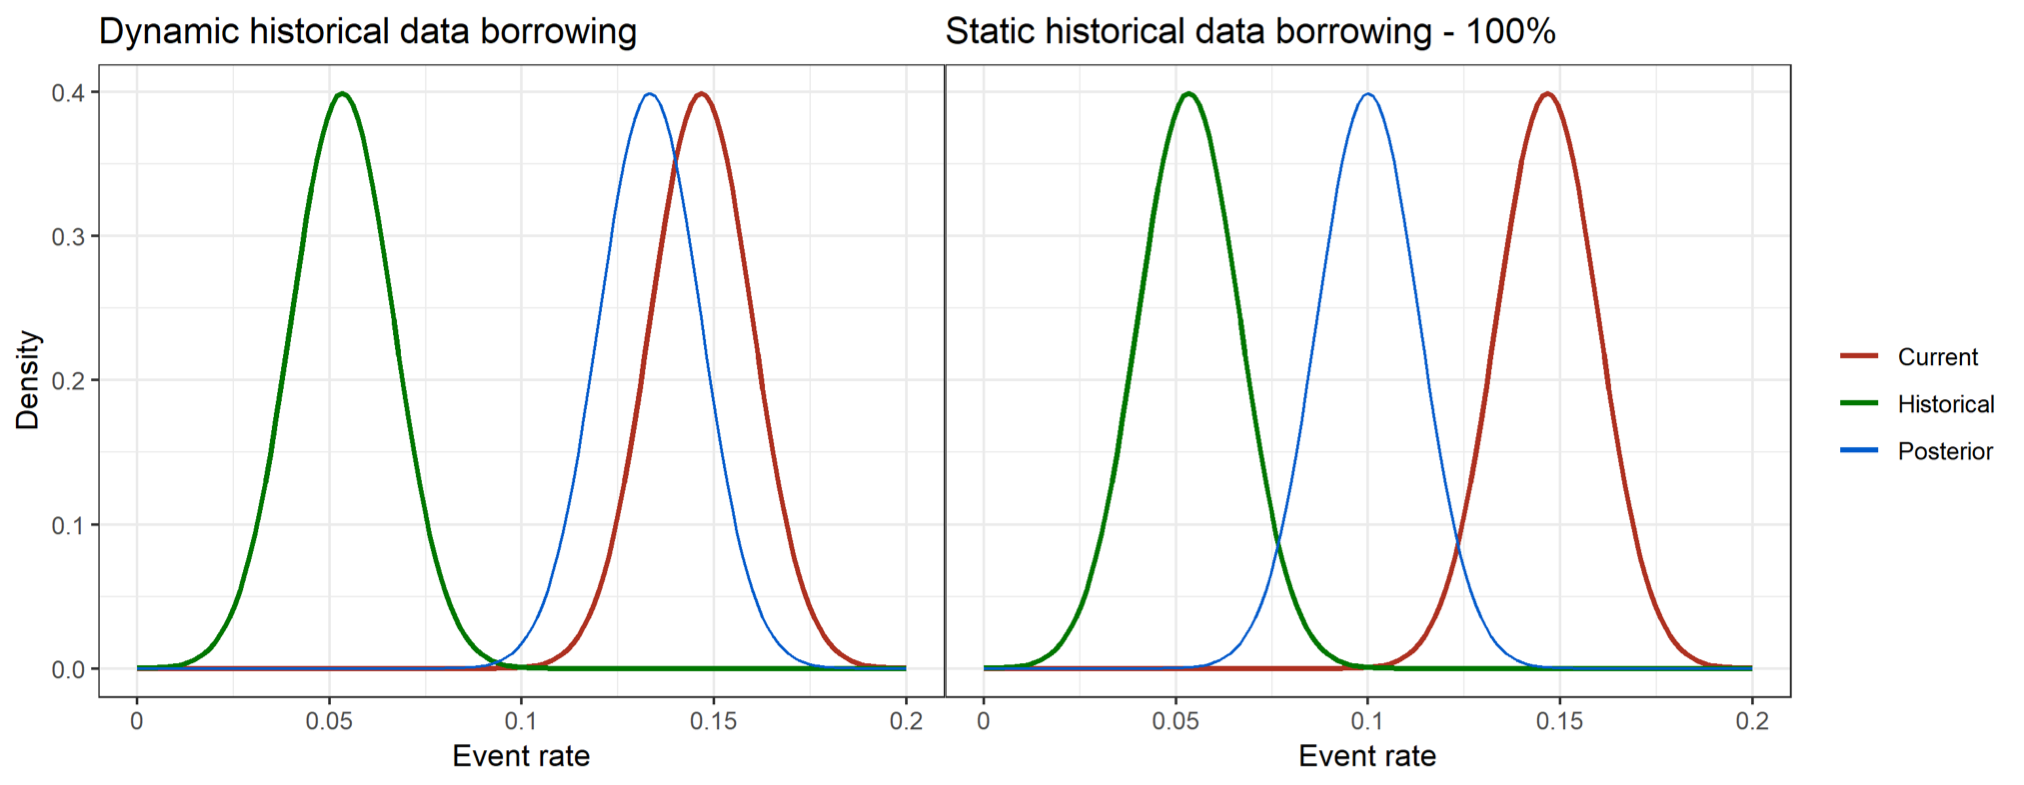
\includegraphics[width=1.1\linewidth]{Images/dynamic.png}}
\end{figure}
\end{frame}





\begin{frame}{Binomial Outcome Example}
\textbf{Single-arm binomial count endpoint with incorporation of historical data}\\
Similar event rates between current and historical data \\
1) Historical data: 28 events in 450 patients \\
2) Current data: 8 events in 200 patients \\
- Carry out estimation via bayesDP:
\begin{figure}
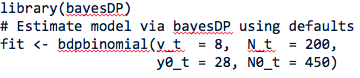
\includegraphics[width=.9\linewidth]{Images/code.png}
\end{figure}

\end{frame}




\begin{frame}{Binomial Outcome Example}
\begin{figure}
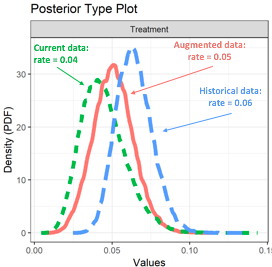
\includegraphics[width=.70\linewidth]{Images/post.png}
\end{figure}
\end{frame}


\section{bayesCT}

\begin{frame}{bayesCT R Package}

\textbf{bayesCT R package available: https://thevaachandereng.github.io/bayesCT/} \\
\begin{itemize}
\item CRAN release 0.99.2 \\
\end{itemize}

\textbf{Analysis types} \\
\begin{itemize}
\item  Single-arm: objective performance criteria trials, treatment data only 
\item Two-arm: treatment + control data 
\end{itemize}

\textbf{Function} \\
\begin{itemize}
\item Incorporation of historical data \\
\item Allow early stopping for futility and expected success \\
\item Pipes for modular input \& parallelization for fast computing \\
\end{itemize}

\end{frame}




%------------------------------------------------

\begin{frame}{Binomial Trial: Single Arm}
Attain Stability Quad Study

$$H_0: \pi_{treatment} \geq 0.08 \qquad H_A:\pi_{treatment} < 0.08$$
\begin{itemize}
\item Lead related complications at 50 days post-implant
\item Enrollment piecewise poisson functions
\item Historical data with 5 failures in 55 samples
\item $Beta(0.5, 0.5)$ prior
\end{itemize}


\end{frame}


%------------------------------------------------

\begin{frame}{Input Parameter}
\begin{figure}
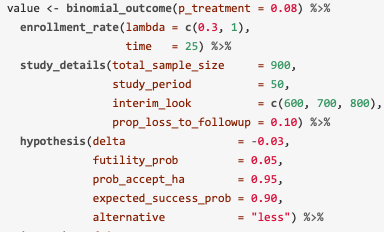
\includegraphics[width=0.9\linewidth]{Images/input1.png}
\end{figure}
\end{frame}

%------------------------------------------------

\begin{frame}{Input Parameter: Continued}
\begin{figure}
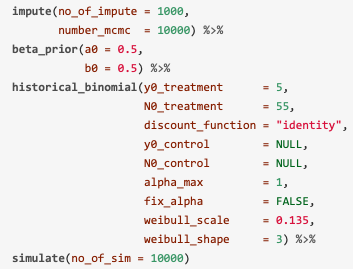
\includegraphics[width=0.8\linewidth]{Images/input2.png}
\end{figure}
\end{frame}

%------------------------------------------------

\begin{frame}{Results}
\begin{table}
  \centering
 \begin{tabular}{|c | c | c |} 
 \hline
Number of  & Power = 0.80 & Power = 0.90 \\ 
Interim Looks & &  \\
 \hline\hline
 1 & (160, 210) & (280, 300)  \\ 
 \hline
 2 & (160, 190, 220) & (280, 300, 310) \\
 \hline
 3 & (160, 180, 210, 230) & (280, 300, 310, 320) \\ [1ex] 
 \hline
\end{tabular}
\caption{Estimated cumulative sample size vectors that provide 80\% and 90\% power for binomial trial from the example and prior of Beta(0.5, 0.5) } \label{tab:simresults}
\end{table}
\end{frame}



%------------------------------------------------

\begin{frame}{bayesCT R Package}

\textbf{Benefits:} \\
\begin{itemize}
\item ease of developing an entire adaptive trial using this package.
\item functions are simple to understand for regulatory agency (FDA).
\item employable for trials with most common data types.
\item ability for a smaller company with a single statistician to be able to develop an entire adaptive clinical trial code.
\item universal language used for describing Bayesian adaptive trials.
\item working on regulatory agency approval!
\end{itemize}
\end{frame}






\section{Future Work}


\begin{frame}{Future Work}
Regulatory agencies (FDA) tend to evaluate proposals for adaptive designs with great scrutiny.
\bi
\itemsep12pt
\item limited exposure with adaptive designs. 
\item concern on the ability of adaptive designs to control type I error.  
\ei
\vspace{24pt}
\onslide<2->{
However, adaptive trials can speed up the drug discovery process rapidly. }

\end{frame}

\begin{frame}{Future Work in RAR}
My future work in RAR will include
\vspace{24pt}
\bi
\itemsep24pt
\item Study multiple treatments rather than 2 treatments.
\item Continuous outcomes.
\ei
\end{frame}


\begin{frame}{Future Work}
My future research work will include 
\bi
\itemsep24pt
\item developing new adaptive designs that alter the inclusion criteria of patients (adaptive enrichment designs).  
\item developing phase II-III seamless designs.
\item creating high-quality open-source computational tools in adaptive designs.
\ei
\end{frame}




\begin{frame}{Acknowledgement}
\bi
\itemsep6pt
\item Rick Chappell (UW-Madison)
\item David DeMets (UW-Madison)
\item Thomas Cook (UW-Madison)
\item Kyungmann Kim (UW-Madison)
\item Donald Musgrove (Medtronic Inc.)
\item Tarek Haddad (Medtronic Inc.)
\item Peter Thall (MD Anderson)
\ei
\end{frame}


\begin{frame}{References}
\bi
\itemsep12pt
\item Karrison TG, Huo D and Chappell R. A group sequential, response-adaptive design for randomized clinical trials. Controlled Clinical Trials 2003; 24(5): 506–522.

\item Thall P, Fox P and Wathen J. Statistical controversies in clinical research: scientific and ethical problems with adaptive randomization in comparative clinical trials. Annals of Oncology 2015; 26(8): 1621–1628.

\item Bashir Q, Munsell MF, Giralt S et al. Randomized phase ii trial comparing two dose levels of thymoglobulin in patients undergoing unrelated donor hematopoietic cell transplant. Leukemia \& lymphoma 2012; 53(5): 915–919.
\ei
\end{frame}

\begin{frame}{References}
\bi
\itemsep12pt
\item Rosenberger WF, Stallard N, IvanovaA et al. Optimal adaptive designs for binary response trials. Biometrics 2001; 57(3): 909–913.

\item Thall PF and Wathen JK. Practical bayesian adaptive randomisation in clinical trials. European Journal of Cancer 2007; 43(5): 859–866.

\item Liu, S., \& Lee, J. J. (2015). An overview of the design and conduct of the BATTLE trials. Chinese clinical oncology, 4(3).

\item Mike V, Krauss AN and Ross GS. Neonatal extracorporeal membrane oxygenation (ecmo): clinical trials and the ethics of evidence. Journal of medical ethics 1993; 19(4): 212–218.
\ei
\end{frame}

\begin{frame}
\vspace{72pt}
\begin {center}
\textbf{THANK YOU!}
\end{center}
\end{frame}


%
%\begin{frame}{Access in action}
%\subt{Interesting reference}
%
%\bigskip
%\centerline{
%\ig[height=0.75\textheight]{Images/img01.jpg}
%}
%
%\note{I'll begin with an illustration of what I mean by
%  access.
%
%  Some time back, I was reading a manuscript and saw an
%  article of interest.}
%\end{frame}
%
%
%\begin{frame}{Access in action}
%\subt{Google Scholar}
%
%\bigskip
%\begin{center}
%\ig[width=0.70\textwidth]{Images/img02.jpg}
%
%\onslide<2> {
%  \vspace*{-0.55\textheight}
%  \hspace*{0.15\textwidth}
%  \ig[width=0.70\textwidth]{Images/img03.jpg}
%}
%\end{center}
%
%\note{If I paste the article title into Google Scholar, I immediately
%  find the paper and can go directly to the journal.
%
%  But I was sitting at home on my couch.
%
%  And they charge \$40 for a 7 page paper!
%
%  I could get the article through the UW Libraries web site, but it's
%  a bit of a hassle.}
%\end{frame}
%
%
%
%
%\begin{frame}{What's the deal with the prices?}
%
%\vspace{24pt}
%
%{\scriptsize \color{gray}
%\renewcommand{\arraystretch}{3}
%\begin{tabular}{p{3.2in}@{\hspace*{1cm}}l}
%Broman K, Speed T, Tigges M ({\color{white} 1996}) Estimation of antigen-responsive T
%cell frequencies in PBMC from human subjects. {\color{white} \mbox{J Immunol Meth}} 198:119{\textendash}132
%& {\color{vhilight} \footnotesize \$39.95}  \\
%Broman KW, Weber JL ({\color{white} 1999}) Method for constructing confidently ordered
%linkage maps. {\color{white} Genet Epidemiol} 16:337{\textendash}343  & {\color{vhilight}
% \footnotesize   \$35.00} \\
%Broman KW, Feingold E ({\color{white} 2004}) SNPs made routine. {\color{white} Nat Methods} 1:104{\textendash}105
%& {\color{vhilight} \footnotesize  \$18.00} \\
%Broman KW ({\color{white} 2005}) Mapping expression in randomized rodent
%genomes. {\color{white} Nat Genet} 37:209{\textendash}210 & {\color{vhilight} \footnotesize  \$18.00}
%\end{tabular}
%}
%
%\note{I went back to some of my early papers, and found these
%  outrageous prices.
%
%  \$18 for a 2-page paper?
%
%  I understand that the publishing industry has a long history of
%  screwy pricing, but you'd have to be either \textbf{desperate} or
%  \textbf{stupid} to pay this.
%
%  And for that 1999 Genetic Epidemiology article, published by Wiley,
%  you have to register in order to find out that it's \$35 for just 24
%  hours of access.
%}
%\end{frame}
%
%
%
%\begin{frame}{Access in action}
%\subt{There's also PubMed}
%
%\bigskip
%\begin{center}
%\ig[width=0.7\textwidth]{Images/img13.png}
%
%
%\onslide<2>{
%  \vspace*{-0.45\textheight}
%  \hspace*{0.55\textwidth}
%  \ig[width=2in]{Images/free_in_pmc.png}
%}
%
%\end{center}
%
%\note{If I'd used PubMed rather than Google Scholar, I could have
%  gotten to the published paper in just a few clicks, because the
%  manuscript is in PubMed Central.
%
%  PubMed Central is only for federally-funded research, has a one year
%  embargo, and (as here) might not include the published version of the
%  paper.
%
%  PubMed Central is a good thing, but one generally can't wait a year,
%  it's unfortunate that the published versions aren't always included,
%  and from an author's point of view it can be a real hassle.
%}
%\end{frame}
%
%
%\begin{frame}{Another example}
%
%\bigskip
%
%\begin{center}
%
%\hspace{-0.15\textwidth}
%\ig[height=0.7\textheight]{Images/feingold_pubmed.png}
%
%\onslide<2->{
%  \vspace*{-0.65\textheight}
%  \hspace*{-0.10\textwidth}
%  \ig[height=0.75\textheight]{Images/feingold_paywall.png}
%}
%
%\onslide<3->{
%  \vspace*{-0.87\textheight}
%  \hspace*{0.38\textwidth}
%  \ig[height=0.92\textheight]{Images/feingold_paper.png}
%}
%
%\onslide<4->{
%  \vspace*{-0.35\textheight}
%  \hspace*{0.29\textwidth}
%  \ig[height=0.35\textheight]{Images/feingold_appendix_url.png}
%}
%
%\onslide<5>{
%  \vspace*{-0.90\textheight}
%  \hspace*{0.48\textwidth}
%  \ig[height=0.85\textheight]{Images/feingold_paywall2.png}
%}
%
%\note{As another example, I was interested a paper from the Journal of
%  Dental Research.
%
%  It's less than a year old, so it's not available in PubMed
%  Central.
%
%  I ordered a copy by inter-library loan, but it didn't include the
%  supplemental methods, and those are behind a paywall at the journal!
%}
%\end{center}
%
%\end{frame}
%
%\begin{frame}{Twitter is useful}
%\subt{(for venting\only<2>{ and more})}
%
%\bigskip
%
%\begin{center}
%
%\ig[height=0.5\textheight]{Images/feingold_tweet.jpg}
%
%\onslide<2->{
%  \vspace*{-0.70\textheight}
%  \hspace*{0.40\textwidth}
%  \ig[height=0.95\textheight]{Images/feingold_appendix.png}
%}
%\end{center}
%
%\note{I was reduced to venting on twitter.
%
%  But then I got the appendix I wanted by email (twice!), within an
%  hour of my tweet. (Thanks, MM and KW!)
%}
%
%\end{frame}
%
%\begin{frame}[c]{Twitter is useful}
%
%\centerline{\Huge {\#}icanhazpdf}
%
%\note{If you search twitter for {\#}icanhazpdf, you'll find lots of
%  people asking for copies of articles. Quite effective.}
%\end{frame}
%
%\begin{frame}{It's all about money}
%\subt{(Costs in scientific publishing)}
%
%\vspace{24pt}
%
%\bi
%\item {\color<3| handout 0>{hilight} Research}
%\item {\color<3| handout 0>{hilight} Writing}
%\item {\color<3| handout 0>{hilight} Peer review, editorial oversight}
%\item {\color<4| handout 0>{hilight} Journal administration}
%\item {\color<4| handout 0>{hilight} Copy editing, typesetting}
%\item {\color<4| handout 0>{hilight} Distribution}
%\item<2-> {\color<2| handout 0>{vhilight} \color<4| handout 0>{hilight} Profit}
%\ei
%
%\note{Open access is all about money.
%
%Most of the costs behind a research paper are paid by grants or
%institutional funds. For most journals, peer review and editorial
%oversight are unpaid.
%
%There are real costs associated with journals, but in the end they are
%all paid from the same sources (grants and institutional funds).
%
%Do we really want to give away the product of our research and then
%buy it back repeatedly, at great profit to the publishers?
%
%And shouldn't the literature be available generally and not just to
%those with access to well-funded research libraries?
%}
%\end{frame}
%
%\begin{frame}{It's not about}
%
%\vspace{36pt}
%
%\bi
%\itemsep6pt
%\item {Peer review}
%\item {Predatory publishing}
%\item {\color<2->{vhilight} Impact factors}
%\item {\color<2->{vhilight} Evaluating researchers} \\
%{\footnotesize \color{gray} (for grants \& promotions)}
%\ei
%
%\vspace{36pt}
%
%\onslide<2->{ \color{hilight} Well, it sort of is\dots }
%
%\note{The Open Access discussion often gets tied up with discussion
%  about peer review, predatory publishing, and journal impact
%  factors.
%
%  But to me, it is a completely separate issue, whether we want
%  stringent peer review before publication or instead leave the
%  evaluation entirely to post-publication review.
%
%  On the other hand, the current culture is to evaluate researchers
%  based on the perceived quality of the journals in which they've
%  published. This makes it difficult to change to open access.
%
%  If everyone's still going to send their best work to Science,
%  Nature, \& Cell, then that work will continue to be locked up behind
%  pay walls.
%}
%\end{frame}
%
%\begin{frame}{Paying for it}
%
%\vspace{36pt}
%
%\bi
%\itemsep12pt
%\item Traditional approach
%\bi
%\item subscriptions
%\item page charges
%\ei
%\item Open access
%\bi
%\item bigger page charges
%\item submission charges?
%\ei
%\onslide<2->{
%\item Endowments
%\item Direct grants to journals
%}
%\ei
%
%\note{The usual way in which publishing costs are paid are through a
%  combination of subscriptions (both institutional and individual) and
%  direct charges to the author.
%
%  In the new open access model, the page charges are increased in
%  order to eliminate the subscription fees. One might have a fee for
%  all submitted manuscripts and not just those accepted for
%  publication.
%
%  I've not seen much discussion of other alternatives, but I would
%  prefer to see endowments established, particularly for
%  society journals.  Alternatively, journals might be
%  funded directly through grants.
%}
%\end{frame}
%
%
%\begin{frame}{Invoice}
%
%\bigskip
%\begin{center}
%\ig[height=0.75\textheight]{Images/invoice3.jpg}
%
%
%\onslide<2>{
%  \vspace*{-0.35\textheight}
%  \ig[width=\textwidth]{Images/invoice3_clip.jpg}
%}
%\end{center}
%
%\note{Here's an invoice for a paper I published in 2012.
%
%  The charges would have been ``just'' \$1700, but I paid an
%  additional \$1200 to have it freely available (otherwise it would
%  have been behind a pay wall for one year).
%}
%\end{frame}
%
%
%
%
%
%
%\begin{frame}{Choices for young investigators}
%
%\vspace{36pt}
%
%\bi
%\item Pay for open access
%\item Support young open access journals
%
%\vspace*{12pt}
%
%\hspace{2cm} {\color{vhilight} \sc or}
%
%\vspace*{12pt}
%
%\item Let subscribers pay \& do more experiments
%\item Continue to go after Science, Nature, \& Cell
%\ei
%
%\note{The page charges, and the continued reliance on impact factors,
%  lead to difficult choices, particularly for young investigators.
%
%  Should I pay for open access, or should I let the subscribers pay
%  and use the savings to do more experiments?
%
%  Should I support open access journals, or should I continue to
%  go after Science, Nature, \& Cell?
%
%  The best scientists may confidently maintain their pure publication
%  record.
%
%  But more mediocre scientists, who may be just scraping by,
%  probably don't feel they have that luxury.  A Nature paper can
%  ``make you.''
%}
%\end{frame}
%
%
%\begin{frame}{What can we do?}
%
%\vspace{36pt}
%
%\bi
%\itemsep12pt
%\item Send our best work to open access journals
%\item Support junior faculty to keep their papers open
%\item Pay attention to the quality of the work
%\bi
%\item[] (not the impact factor of the journal)
%\ei
%\item Raise endowments for trusted journals
%\item {\color<2>{vhilight} Reform copyright law}
%\ei
%
%\note{We need to send our best work to open access journals.
%
%We need to find ways to support our junior colleagues, so that they
%may do so as well.
%
%We need to evaluate people based on their work and not by the name of
%the journal in which it appeared. We all may say, ``Science and
%Nature are often crap and there are lots of fantastic papers that
%appear elsewhere.'' But somehow when we see Nature or Cell on
%someone's CV, we still have an immediate, positive reaction.
%
%I would like to see endowed journals, open forever.
%
%The quickest way to free the product of federally funded research
%would be to reform copyright law. If the product of our research were
%forced open by law, the publishing industry would figure out how to
%pay for it in short order.
%
%But given the state of politics in the US, I'm not too optimistic
%about that.
%}
%\end{frame}
%
%{\setbeamertemplate{footline}{}
%
%\begin{frame}
%\end{frame}
%
%\begin{frame}{Discussion questions}
%
%\vspace{12pt}
%
%{\small
%\bi
%\itemsep12pt
%    \item {\color{lolight} \footnotesize There is an emerging consensus to allow (or
%      even require) self-archiving for the final version of the
%      author's peer-reviewed manuscript, and to give the publisher
%      exclusivity for the published edition.} \\
%      Is this a problem for the researchers that use the content?
%    \item How to encourage researchers to publish in open access
%      journals? How to help with publication charges?
%    \item Should we change how we evaluate scholars, for hiring and
%      promotion?
%    \item Should we give campus authors a chance to "opt-out" of any
%      institutional mandate for open access?
%  \ei
%}
%
%\end{frame}

%}
\end{document}
